\newtoggle{test-minted}
%\toggletrue{test-minted}

\section{Text}

Regular text.?! 0-123+456*789/0

\texttt{ Monospace text.?! 0-123+456*789/0!}

\textit{ Italic text.?! 0-123+456*789/0!}

\textbf{ Bold text.?! 0-123+456*789/0!}

\section{Math Equations}\label{math-equations}

You may want to display math equations in three distinct styles: inline,
numbered or non-numbered display. Each of the three are discussed in the
next sections.

\subsection{Inline (In-text) Equations}\label{inline-in-text-equations}

A formula that appears in the running text is called an inline or
in-text formula. It is produced by the \textbf{math} environment, which
can be invoked with the usual
\texttt{\textbackslash{}begin,\ ...\ \textbackslash{}end} construction
or with the short form
\texttt{\textbackslash{}\$\ ...\ \textbackslash{}\$}. You can use any of
the symbols and structures, from \(\alpha\) to \(\omega\), this section will simply show a few
examples of in-text equations in context. Notice how this equation:
\(\lim_{n\rightarrow \infty}x=0\), set here in in-line math style, looks
slightly different when set in display style. (See next section).

\subsection{Display Equations}\label{display-equations}

A numbered display equation---one set off by vertical space from the
text and centered horizontally---is produced by the \textbf{equation}
environment. An unnumbered display equation is produced by the
\textbf{displaymath} environment.

Again, in either environment, you can use any of the symbols and
structures available in \LaTeX@; this section will just give a couple of
examples of display equations in context. First, consider
Equation~\ref{eq-oneequation}, shown as an inline equation above:

\begin{equation}\phantomsection{
\lim_{n\rightarrow \infty}x=0
}\label{eq-oneequation}\end{equation}

Notice how it is formatted somewhat differently in the
\texttt{displaymath} environment. Now, we'll enter an unnumbered
equation:

\[\sum_{i=0}^{\infty} x + 1\]

Note some fine points concerning \texttt{mathit} and
how math and text fonts are different sometimes.

\begin{center}
  \begin{tabular}[c]{|l|l|l|l|}
    just math & $brown~fox$ \\
    \texttt{mathit} & $\mathit{brown~fox}$ \\
    \texttt{textit} & $\textit{brown~fox}$ \\
    \texttt{textbf}& \textbf{brown~fox} \\
    \texttt{mathbf}& $\mathbf{brown~fox}$ \\
    \texttt{mathrm}& $\mathrm{brown~fox}$ \\
    \texttt{textrm}& \textrm{brown~fox} \\
    \texttt{boldsymbol}& $\boldsymbol{brown~fox}$ & $\boldsymbol{\partial\times\sum_i}$\\
              && $\partial\times\sum_i$&just math \\
    text mono spaced& s\texttt{st}t &\\
    math mono spaced& $\mathrm{s}\mathtt{st}\mathrm{t}$&
  \end{tabular}
\end{center}

\subsubsection{More information}

A numbered display equation---one set off by vertical space from the
text and centered horizontally---is produced by the \textbf{equation}
environment. An unnumbered display equation is produced by the
\textbf{displaymath} environment.

\paragraph{Further details}

Again, in either environment, you can use any of the symbols and
structures available in \LaTeX@; this section will just give a couple of
examples of display equations in context. First, consider
~\eqref{eq-oneequation}, shown as an inline equation above:

\section{Math Tests}

\begin{definition}[name={Heterogeneous Validity \protect\citep{anoma-taiga}}, label={def:het-valid}]
    A consensus execution\todo{take Guerraoui definition for what an execution is}
    is \emph{valid} if all  decided values were proposed in that execution.
    A consensus protocol is \emph{valid} if all possible executions are valid.
\end{definition}

Characterization of the Imaginary Forms
Theorem.
Let $S=\left\{v_1, v_2, \ldots, v_k\right\}$ be a set of vectors in $\mathbb{R}^n$.

% \begin{center}
% |"|πκομπ̈ρέσα, αντιανταντ ̈ ικός, ελεγκ ̈ τής
% \end{center}

\begin{center}
    $\perp$
    \begin{equation}
        \begin{split}
        &(\mathit{Blue}, \mathit{Red})\\
        &\mathcal{ABC DEF GHI JKL MNO PQR ST UVW XYZ}\\
        &\mathbb{ABC DEF GHI JKL MNO PQR ST UVW XYZ}\\
        &\mathfrak{ABC DEF GHI JKL MNO PQR ST UVW XYZ}\\
        &\mathscr{ABC DEF GHI JKL MNO PQR ST UVW XYZ}\\
        \end{split}
    \end{equation}
\end{center}
%\renewcommand{\operatorname}[1]{\mathop{\text{#1}}}
Consider $\mathcal{F}(S)=\sum_{i=1}^k \delta\left(v_i v_j w\right) \sigma_{i, j}$.
If $\mathcal{F}(S) \leq \varepsilon$, then
$$
\phi(S, \alpha)=\frac{1}{2 \pi i} \int_{-\infty}^{753} \frac{\tilde{W}_n(\gamma) \cos \left(\sqrt{x^2}\right)}{f^{\prime}(x) R / a} d x=\operatorname{det}\left(\begin{array}{cc}
\alpha^2 & \Pi \\
\omega & x \otimes y
\end{array}\right)
$$


Note: If $\beta \in \Gamma$, then the form is undefined at the points in $S \cap \Gamma$, and the integral $l_l\left(i_1\right)$ diverges as $\varepsilon \rightarrow 0$. This pathological behavior can be handled by taking $\Gamma \subseteq S$.

\iftoggle{test-minted}{
{
  \small
\begin{minted}{python}
def even_constraint(last_state, next_state_var, solver):
    n = solver.IntVar(0, solver.infinity(), 'n_even')
    b = solver.BoolVar('b_even')
    solver.Add(next_state_var - 2 * n <= M * (1 - b))
    solver.Add(next_state_var - 2 * n >= -M * (1 - b))
    return [(b, 1)]
\end{minted}
}
}{}

\begin{comment}

\begin{betterpython}
    def even_constraint(last_state, next_state_var, solver):
        n = solver.IntVar(0, solver.infinity(), 'n_even')
        b = solver.BoolVar('b_even')
        solver.Add(next_state_var - 2 * n <= M * (1 - b))
        solver.Add(next_state_var - 2 * n >= -M * (1 - b))
        return [(b, 1)]
\end{betterpython}

\begin{lstlisting}{python}
    def odd_constraint(last_state, next_state_var, solver):
        n = solver.IntVar(0, solver.infinity(), 'n_odd')
        b = solver.BoolVar('b_odd')
        solver.Add(next_state_var - 2 * n - 1 <= M * (1 - b))
        solver.Add(next_state_var - 2 * n - 1 >= -M * (1 - b))
        return [(b, 1)]
\end{lstlisting}

\end{comment}
Graph three coloring is a common example used to introduce CSPs to new audiences. The goal is to color the nodes of a graph with three colors such that no two same-colored nodes touch. 

\begin{equation}
    \forall c \in C, t \in E_{G, c}, \quad \prod_{i<a(c)} f_V(t_i) \in E_{H, c}.    
\end{equation}


\begin{equation}
    \sum_{i=0}^\infty c \in C, t \in E_{G, c}, \quad \int_{i<a(c)} f_V(t_i) \in E_{H, c}.    
\end{equation}

The CSP itself consists of a single binary relation asserting the inequality between three elements, typically named after primary colors.

\begin{equation}\label{equation:three-color-neq-def}
  \neq\ = \{ (\mathit{Blue}, \mathit{Red}), (\mathit{Blue}, \mathit{Green}), (\mathit{Red}, \mathit{Blue}), (\mathit{Red}, \mathit{Green}), (\mathit{Green}, \mathit{Blue}) \}
\end{equation}

Graphs become instances by translating edges into binary relations. Take this graph as an example;

\begin{center}
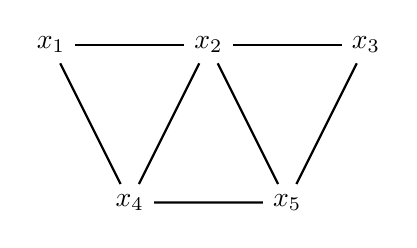
\begin{tikzpicture}[thick]
  \node (A) at (0,0) {$x_1$};
  \node (B) at (2,0) {$x_2$};
  \node (C) at (4,0) {$x_3$};
  \node (D) at (1,-2) {$x_4$};
  \node (E) at (3,-2) {$x_5$};

  \draw (A) -- (B) -- (C);
  \draw (A) -- (D) -- (E) -- (C);
  \draw (D) -- (B);
  \draw (E) -- (B);
\end{tikzpicture}
\end{center}

\subsection{Corresponding CSP instance}

We can simply list the edges using the inequality relation to produce the corresponding CSP instance;

\begin{equation}
    x_1 \neq x_2 \wedge x_1 \neq x_4 \wedge x_2 \neq x_3 \wedge x_2 \neq x_4 \wedge x_2 \neq x_5 \wedge x_3 \neq x_5 \wedge x_4 \neq x_5
\end{equation}

A solution to the graph coloring problem is then an assignment of colors that satisfies the instance. 


\begin{table*}[!h]
\begin{center}
\begin{tabular}{p{1.5cm}p{13cm}}
\toprule
  \textbf{Role} & \textbf{Description} \\
\midrule
  Authorizer & approves the resource consumption on the application level. The resource logic encodes the mechanism that connects the authorizer's external identity (public key) to the decision-making process 
  \\
  Annuler & knows the data required to nullify a resource
  \\
  Creator & creates the resource and shares the data with the receiver
  \\
  Owner & can both authorize and annul a resource
  \\
  Sender & owns the resources that were consumed to create the created resource
  \\
  Receiver & owns the created resource
  \\
\bottomrule
\end{tabular}
\caption{Resource-related roles.}
\end{center}
\end{table*}


If we think about the structure of this graph, we notice that it has three triangles, the left and right side triangles $(x_1, x_2, x_4)$  and $(x_2, x_3, x_5)$, and the central triangle $(x_2, x_4, x_5)$. Each must be a triple of distinctly colored points. The edge between $x_4$ and $x_5$ forces those two to have distinct colors, while the two side triangles share a color at $x_2$. These two observations force us to conclude that the left triangle has the colors of the right triangle flipped along the bisector going through $x_2$. If we arbitrarily select $x_1$ to be $\mathit{Blue}$ and $x_2$ to be $\mathit{Red}$, we are then forced into the coloring;

\begin{equation}
 \langle x_1 \rightarrow \mathit{Blue}; x_2 \rightarrow \mathit{Red}; x_3 \rightarrow \mathit{Green}; x_4 \rightarrow \mathit{Green}; x_5 \rightarrow \mathit{Blue}\rangle,
\end{equation}

which will satisfy this instance. We can place these colors back on the graph to verify the solution visually.

Citations are also possible, for example: \citep{christopher_goes_2023_8279842}
